\chapter{Data management}

Previously, it was shown how to manipulate surfaces, masks for segmentation and measurements. It is possible to show or
hide, and create or remove these elements at the \textbf{Data} management panel, located in the left inferior corner of
Invesalius. The panel is divided in 3 tabs: \textbf{Masks}, \textbf{3D Surfaces} and \textbf{Measurements}, shown in
figure \ref{fig:volumetric_data}. Each tab contains features corresponding to the elements it referes to.

\begin{figure}[!htb]
\centering
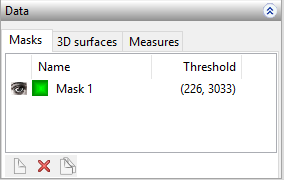
\includegraphics[scale=0.7]{painel_mask_manager_en.png}
\caption{Data management}
\label{fig:volumetric_data}
\end{figure}

In each tab, there is a panel divided in rows and columns. First column of each line determines the visualization status
of the listed element. It means that the "eye" icon activates or deactivates the masks, surface or measurement exibition.
In case one of these elements is being exhibited, its corresponding icon shown in figure \ref{fig:disable_mask}, will
also be visible.

\newpage

\begin{figure}[!htb]
\centering
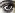
\includegraphics[scale=0.9]{eye}
\caption{Icon indicating the elements visibility}
\label{fig:disable_mask}
\end{figure}

Some operations may be porformed with the data. For instance, to remove one element, it is necessary to first select
its name, show in figure \ref{fig:selected_mask} and next click in the shortcut illustrated in
figure \ref{fig:delete_data}.

\begin{figure}[!htb]
\centering
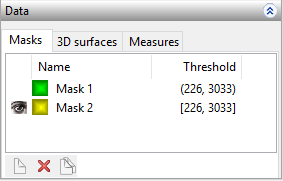
\includegraphics[scale=0.7]{painel_selected_mask_en.png}
\caption{Data selected}
\label{fig:selected_mask}
\end{figure}


\begin{figure}[!htb]
\centering

\includegraphics[scale=0.8]{data_remove.png}
\caption{Remove data}
\label{fig:delete_data}
\end{figure}

To create a new mask, surface or measurement, click in the shortcut show in figure \ref{fig:new_data}, considering that
the corresponding tab must be open.

\begin{figure}[!htb]
\centering

\includegraphics[scale=0.8]{data_new.png}
\caption{New data}
\label{fig:new_data}
\end{figure}

To duplicate a data, select it and click in the shortcut shown in figure \ref{fig:duplicate_data}.

\begin{figure}[!htb]
\centering

\includegraphics[scale=0.8]{data_duplicate.png}
\caption{Duplicate data}
\label{fig:duplicate_data}
\end{figure}


\newpage


\section{Masks}

At column \textbf{Name}, the mask's color and name are show. In turn, column \textbf{Threshold} show the value range
used to create the mask. Figure \ref{fig:volumetric_data} exhibits an example.

\section{3D Surface}

At column \textbf{Name}, the surface's color and name are show. Column \textbf{Volume} show the total surface volume.
Finally, column \textbf{Transparency} indicates the level of transparency in use for surface visualization.
Figure \ref{fig:surface_manager} shows an example.

\begin{figure}[!htb]
\centering
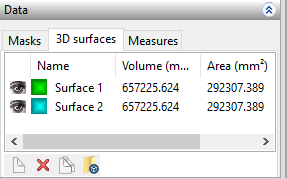
\includegraphics[scale=0.7]{painel_volumetric_measures_en.png}
\caption{Surface manager}
\label{fig:surface_manager}
\end{figure}

\subsection{Import surface}

It is possible to import a file of type STL, OBJ, PLY or VTP (VTK Polydata File Format) with an active InVesalius
project. To do so, click in the icon shown in figure~\ref{fig:import_stl}, select the
format of the corresponding file, figure~\ref{fig:import_surface}, and click Open.

\begin{figure}[!htb]
\centering

\includegraphics[scale=0.8]{load_mesh.png}
\caption{Shortcut to import surface }
\label{fig:import_stl}
\end{figure}

\begin{figure}[!htb]
\centering
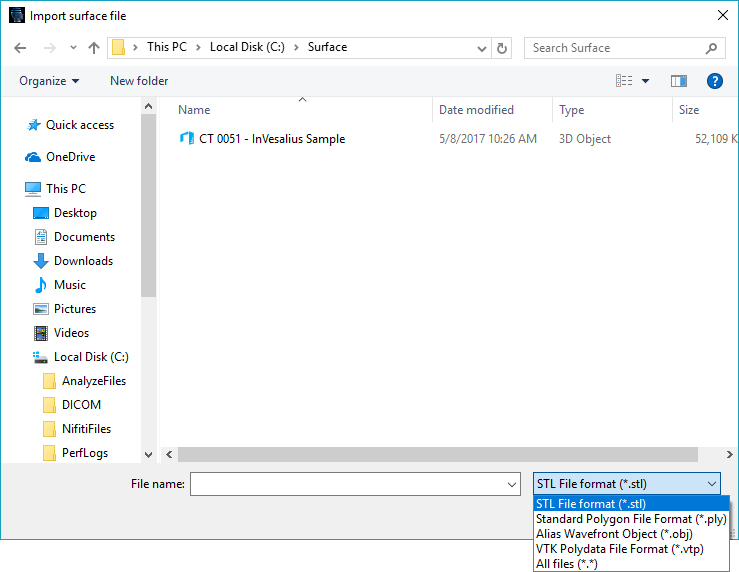
\includegraphics[scale=0.4]{import_surface_en.png}
\caption{Window to import surface}
\label{fig:import_surface}
\end{figure}

\newpage


\section{Measurements}

The tab \textbf{Measurements} shows the following information. Column \textbf{Name} indicates the color and measurement
name. Column \textbf{Local} indicates where the measurement was taken (image axial, coronal, sagital or 3D), and
\textbf{Type} indicates the type of measurement (linear or angular). Finally, column \textbf{Value} shows the
measurement value. Figure \ref{fig:manager_mensuares} illustrates the \textbf{Measurements} tab.

\begin{figure}[!htb]
\centering
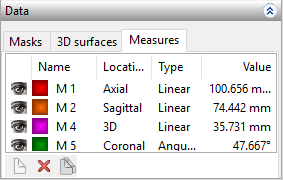
\includegraphics[scale=0.7]{painel_measures_manager_en.png}
\caption{Data management}
\label{fig:manager_mensuares}
\end{figure}

